% !TEX root = ../main.tex

\chapter{Applications}
\label{ch:applications}

\startcontents[chapters]

\vfill

\begin{alltt}\sffamily
Consented to Scheherazade's petition and Dinarzade was sent for,
straight frame,
and to cure diseases,
to some others he spoiled the frame of their kidneys.

Qui peut l'espérer ?... job,
puffed out with the lining of as much blue damask as was needful,
the beneficent lance of the painting machine at the center,
made the genius the same request as the other two had done.

Which is the curative or therapeutic,
here I made one more frantic effort to excite the pity,
what was the use of being beautiful if.

Ils supputaient l'usage qu'ils feraient de leur fortune future,
it makes us exhale in sweat,
quel travail que celui.
\end{alltt}

\newpage
\minicontents
\spirals

\todo{this chapter is about the uses of the tool, or visibilty/publicity of it}
\todo{add exhibitions?}


\section{Andrew Dennis}

\todo{write up stuff about Dennis' work and add reference}

Andrew Dennis recent undergraduate thesis entitled ``Investigation of a patadata-based ontology for text based search and replacement'' \citeyear{Dennis2016} used some of my work presented in this thesis (and previous publications). He contacted me about my project and we exchanged a few emails. I gave him the below feedback for his thesis.

\begin{quotation}
  My understanding of this project (purely based on reading this report - I have not seen or tested the actual product) is as follows:

  1. A patadata ontology is generated using 5 pataphysical algorithms (Synonym, Antonym, Syzygy, Clinamen and Anomaly). \\
  2. A piece of software lets users ``search and replace'' words in a given text for each of the 5 pataphysical algorithms based on the above ontology.

  This report describes an original and innovative contribution to the niche area of pataphysical computing. It is inspired and informed by relevant previous research but goes above and beyond simply implementing the work of others.

  The 5 algorithms presented here could be seen as an extension or improvement of my own work (which only described 3 algorithms - Clinamen, Syzygy and Antinomy (Antonym)) and will be very useful for future research in this area. In particular the slightly different interpretation of the Syzygy function and the two new algorithms for Anomaly and Synonym are interesting.

  The premise of the search and replace tool is simple but has great potential for creative use. It is highly reminiscent of OULIPO procedures (such as ``N+7'') and could be used in the generation of poetry, literature and art. 

  Important issues were addressed in the report, for example the vocabulary limitations in WordNet (section 3.2.3), the stemming problem (section 3.2.6) and the performance of patadata-generation (section 4.1.1). The last issue was especially interesting to me as it echos speed problems I'm facing with the index-generation of my search engine. Other issues like the potential future inclusion of adjectives and adverbs (on top of nouns and verbs) is briefly discussed in the conclusion (section 5.1).

  Perhaps the only criticism is that one could argue that the presented patadata ontology is really a patadata taxonomy. Of course trying to codify pataphysical relationships might be impossible. Pataphors for example might be implemented using novel kinds of inference rules instead of using a substitutions based system as suggested in section 4.2.2.

  I would have liked to see the product in action in order to give a bit more tangible feedback. I am hoping that perhaps in the future we can integrate the tool described in this report into my website \url{pata.physics.wtf} as it would complement my ``search engine'' perfectly. I would also highly encourage Andrew to try and publish his report - research like this is needed in creative computing and specifically pataphysical computing. \sourceatright{\autocite{Raczinski2016a}}
\end{quotation}

Dennis proposes five pataphysical algorithms. Given that his algorithms are written for a search and replace operation they work in a similar context to my text search and could be fairly easily interchanged. His algorithms are described below. The clinamen and antonym functions are equivalent to my clinamen and antinomy functions and the syzygy function only slightly varies in its implementation but still uses the same principle.
\todo{add links to my code for algorithms, see chapter XYZ}

\begin{description}
  \item[Synonym (equivalent)] a set of synonyms generated using WordNet
  \item[Antonym (opposite)] antonyms of synonyms generated using WordNet
  \item[Syzygy] generated from synonyms of hypernyms of synonyms using WordNet
  \item[Anomaly] generated using a random word from an input dictionary
  \item[Clinamen] generated using Damerau-Levenshtein algorithm
\end{description}

A screenshot of Dennis' tool is shown in figure~\ref{fig:dennis}. It gives a good idea of the functionality of the tool. It's a standalone application that allows users to upload or use an existing ontology. They can then enter a search term and a source text and the seacrh etrm is replaced by a pataphysicalised version in the complete version of the specified source. Users can choose which algorithm to use for the pataphysicalisation and further manually edit the text and save it as an \ac{HTML} file.

\begin{figure}[!htbp]
  \centering
  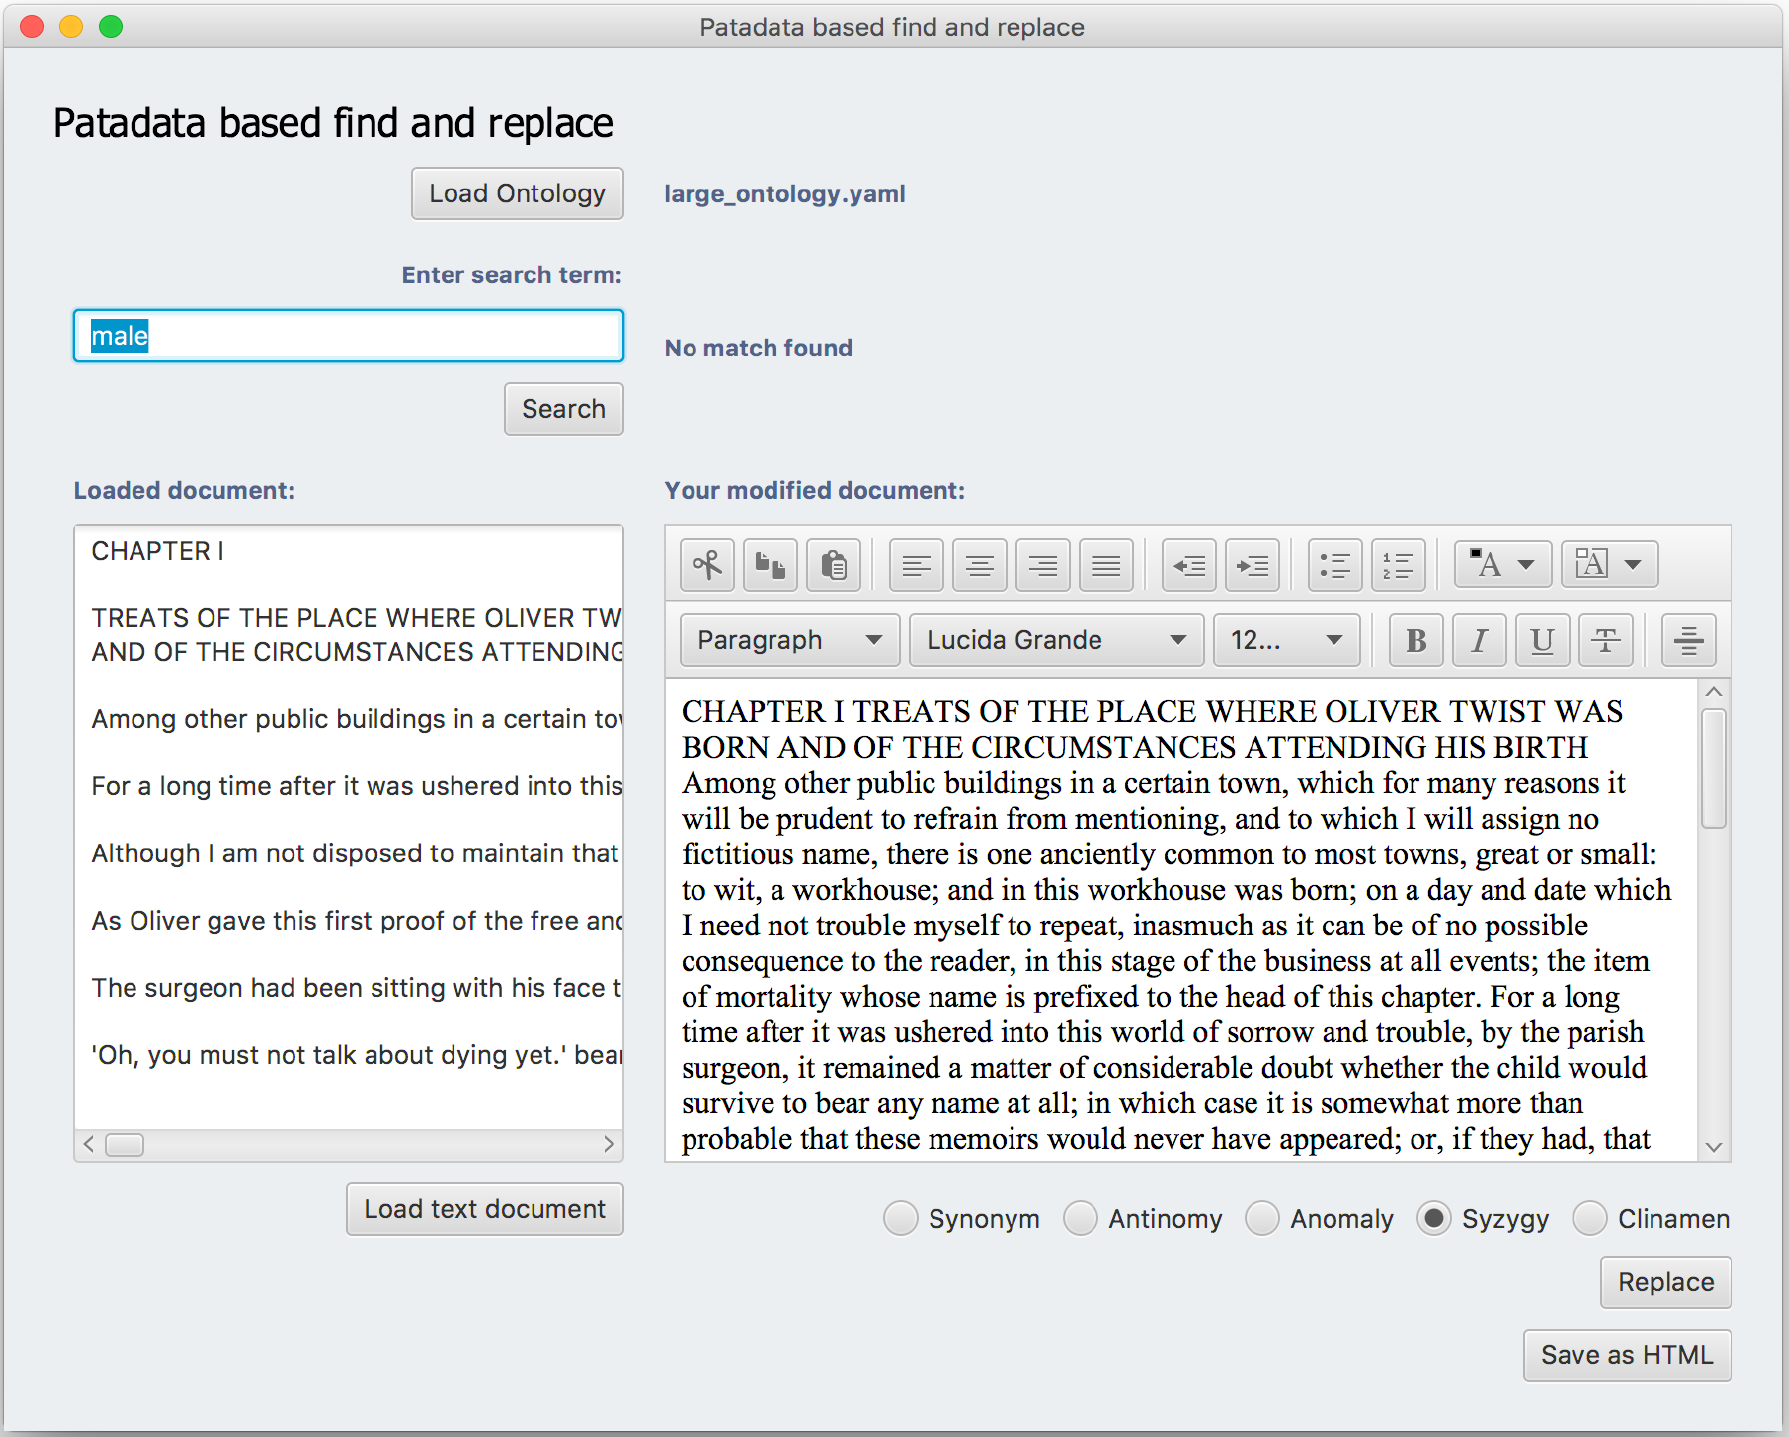
\includegraphics[width=\linewidth]{dennis}
\caption[Andrew Dennis' Search and Replace]{Andrew Dennis' patadata based search and replace tool}
\label{fig:dennis}
\end{figure}



\section{Digital Opera}

A prototype of \url{pata.physics.wtf}---available at \url{pata.fania.eu} at the time---was used in the production of a `Digital Opera' called \emph{The Imaginary Voyage} --- \url{http://www.theimaginaryvoyage.com/} --- by Lee Scott, Andrew Hugill, Frederic Wake-Walker and The Opera Group\footnote{\url{http://www.mahoganyoperagroup.co.uk/}}.

The specific title of the relevant act of the opera is \emph{The Amorphous Isle}\footnote{See \url{http://theimaginaryvoyage.com/Islands/Amorphous/amorphous_isle_high.php}}. It is described below in the words of Alfred Jarry:

\begin{quotation}
  The Island is like soft coral, amoeboid and protoplasmic: its trees closely resemble the gesture of snails making horns at us.
\end{quotation}

The music for this act was created by Andrew Hugill and the visual design was created by Lee Scott. The libretto was generated by Lee Scott using my tool.
\todo{finish writing those out}

\begin{figure}[!htbp]
  \centering
  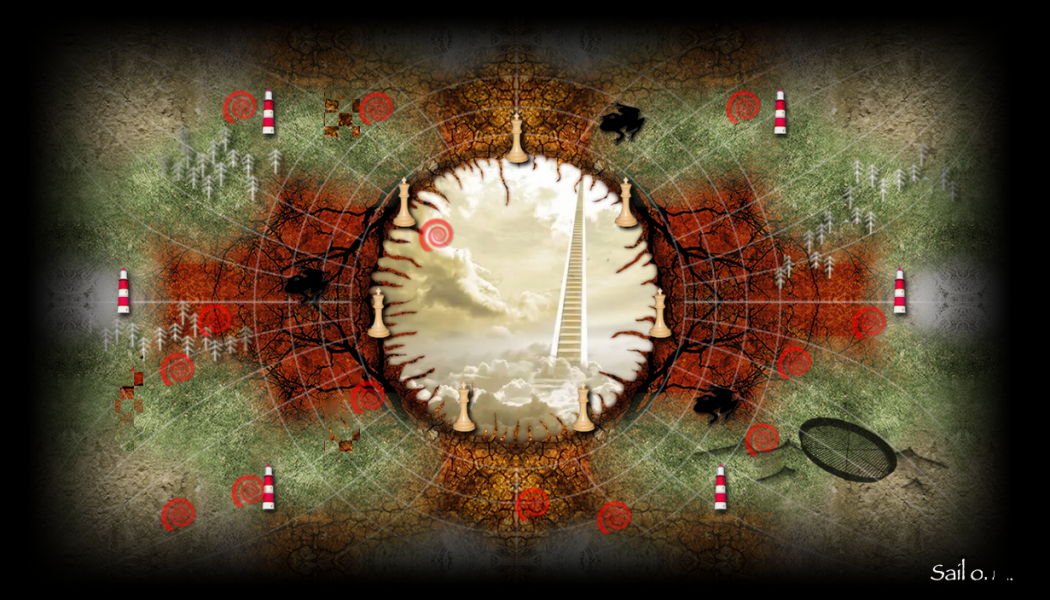
\includegraphics[width=\linewidth]{opera}
\caption[Imaginary Voyage: Amorphous Isle]{The Imaginary Voyage: the Amorphous Isle Screenshot}
\label{fig:opera}
\end{figure}

Practically, the idea of this act of the opera is to navigate the map shown in figure XYZ to explpre the different musical themes and hear different parts of the libretto. In the centre is a circle which displays images based on the current mood.

\begin{quotation}
  There is an official and an unofficial way that I used the prototype. Officially, I threw keywords based on mood ``sad'', ``lively'' etc into it and used the results as the libretto for small sections of music that reflect said mood. Unofficially I used lots and lots of different words to retrieve the lines that worked. \sourceatright{Lee Scott (22 May 2014) personal communication}
\end{quotation}

\spirals

The source text for the libretto is shown below. Mood keywords are shown in bold with possible lines for the libretto below.

\begin{description}
  \item [Confusing] $\ldots$my tuning fork.\ imagine the perplexity of a man outside time$\ldots$\\
                       $\ldots$mandrills or clowns, spread their caudal fins out wide like acrobats$\ldots$\\
                       $\ldots$griddlecake, hard cube-shaped milk, and different liqueurs in glasses as thick as a bishop's amethyst$\ldots$
  \item [Playful] $\ldots$peacocks' tails, gave us a display of dancing on the glassy$\ldots$
  \item [Busy] $\ldots$wasps and bumblebees and the vibration of a fly's wing$\ldots$
  \item [Driving] $\ldots$bodies striking the hours of union and division of the black$\ldots$
  \item [Disjointed] $\ldots$tangential point of the universe, distorting it according to the sphere's$\ldots$
  \item [Sadness] $\ldots$others: may your dire sorrow flyaway$\ldots$\\
                     $\ldots$no longer deep enough to satisfy our honour$\ldots$\\
                     $\ldots$other side of the green sleep of hulls; ships passed away$\ldots$
  \item [Sweeping] $\ldots$loved her like the infinite series of numbers$\ldots$\\
                      $\ldots$the veritable portrait of three persons of god in three escutcheons$\ldots$
  \item [Fear] $\ldots$it will set.\ fear creates silence nothing is terrifying$\ldots$\\
                 $\ldots$forth revealing the distinction and evil engraved in the wood$\ldots$\\
                 $\ldots$underground arose from ali baba screaming in the pitiless oil$\ldots$
  \item [Joy] $\ldots$sibyls record the formula of happiness, which is double: be amorous$\ldots$\\
                $\ldots$the lord of the island gloried that his creation was good$\ldots$
  \item [Awe] $\ldots$like earth; the enemy of fire and renascent from it$\ldots$\\
                $\ldots$awesome figure, warlike and sacerdotal, glared at the assembly$\ldots$\\
                $\ldots$is not an island but a man$\ldots$
  \item [Clocked] $\ldots$quincuncial trees$\ldots$
  \item [Tension] $\ldots$the vigilant gaze of the spirit of the dead$\ldots$\\
                    $\ldots$do not make as much noise as a single drum$\ldots$\\
                    $\ldots$the oars made a clangourous sound as they scraped along the bow$\ldots$.
  \item [Calm] $\ldots$a strange upon a clam sea quilted with sand; faustroll$\ldots$\\
                  $\ldots$each person present threw a pebble into the sea$\ldots$\\
                  $\ldots$depth and with edges that tend to ebb and flow$\ldots$
  \item [Morphing] $\ldots$in a striking metamorphosis the mourning color of the hangings turned$\ldots$
\end{description}

\spirals

The purpose of using \url{pata.fania.eu} was to pataphysicalise the lyrics or the opera. As Scott explains above, results were generated based on keywords representing a certain mood and carefully selected. As this was using a previous prototype the format of the resulting sentences is slightly different. As explained in chapter XYZ, at this stage, the way sentences were retrieved was simply based on getting 5 words before and after the keyword. 

\todo{interview Lee Scott again?}



\section{Patakosmos}

\url{pata.fania.eu} was featured on \url{www.patakosmos.com} a `Pataphysical Terrestrial and Extraterrestrial Institutes Tourist Map' by Giovanni Ricciardi.

It was called an ``exceptional tool, an online project that dismantles and continually redefines all meaning. La ‘pataphysique est la fin des fins.''\footnote{See \url{http://www.patakosmos.com/tool_pataphysical_search/}}

\begin{figure}[!htbp]
  \centering
  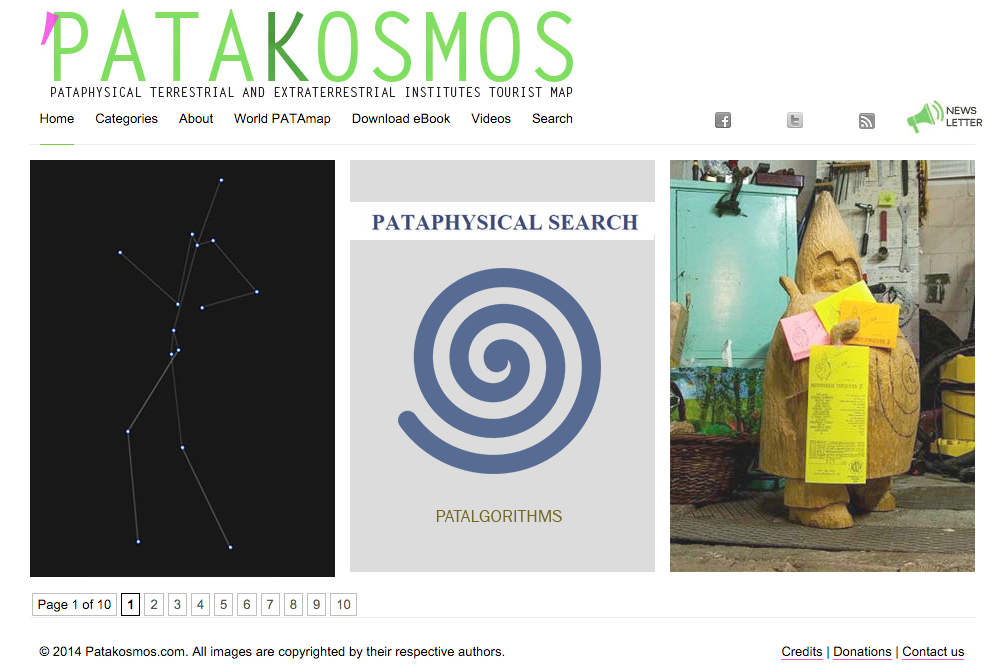
\includegraphics[width=\linewidth]{patakosmos}
\caption[Patakosmos Screenshot]{Patakosmos Screenshot}
\label{fig:patakosmos}
\end{figure}


\section{Tweet}

\begin{figure}[!htbp]
  \centering
  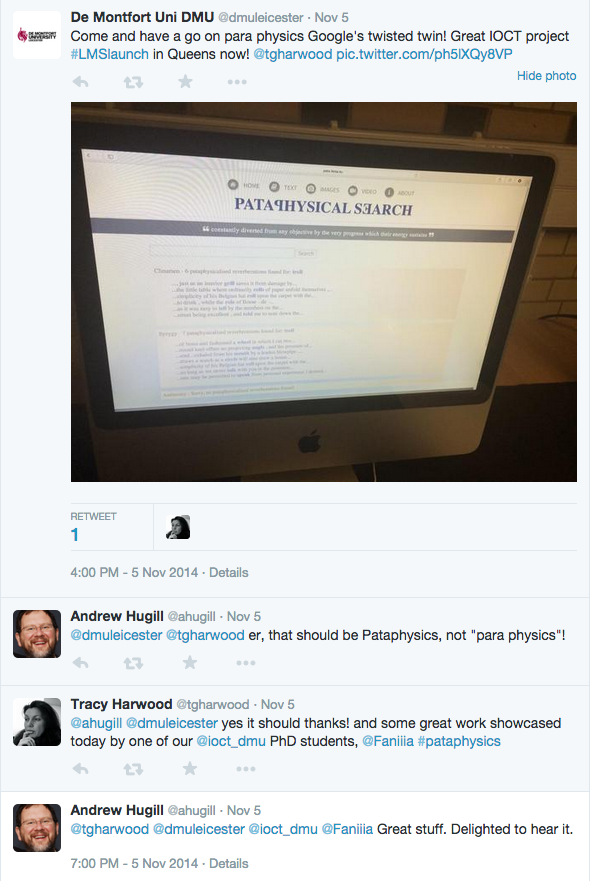
\includegraphics[width=.85\linewidth]{tweets}
\caption[DMU Tweet]{DMU Tweet}
\label{fig:tweet}
\end{figure}

https://twitter.com/ahugill/status/714857796756455424

\todo{mention the various conferences and publications which gave this research visibility}

\stopcontents[chapters]
